
\begin{figure}
\centering
\begin{subfigure}{.5\textwidth}
  \centering
  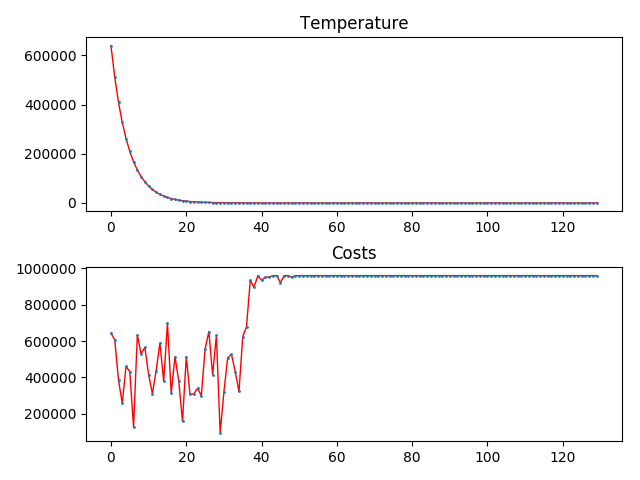
\includegraphics[width=1\linewidth]{results/cut12/2/plot}
  \label{fig:sub1}
\end{subfigure}%
\begin{subfigure}{.5\textwidth}
  \centering
  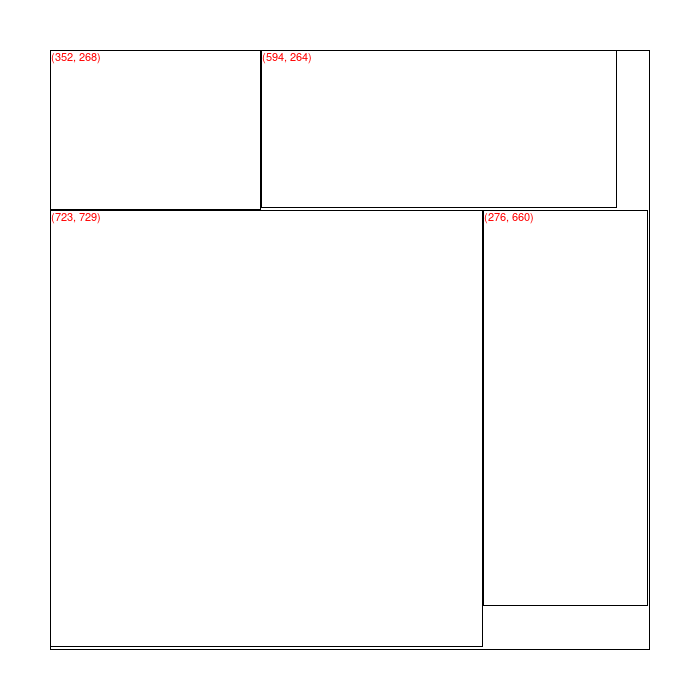
\includegraphics[width=1\linewidth]{results/cut12/2/cut}
  \label{fig:sub2}
\end{subfigure}
\caption{Instancia cut12.txt, Solução: 960379, disperdício de 3.96\% de 1000x1000, {(594, 264): 1, (723, 729): 1, (276, 660): 1, (352, 268): 1}}
\label{fig:test}
\end{figure}


\begin{figure}
\centering
\begin{subfigure}{.5\textwidth}
  \centering
  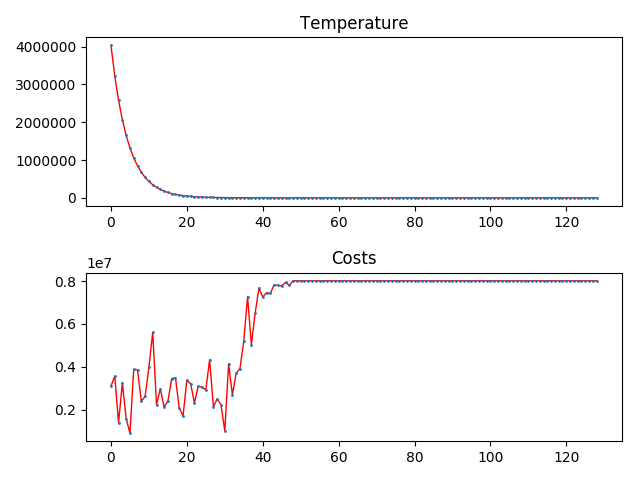
\includegraphics[width=1\linewidth]{results/cut13/2/plot}
  \label{fig:sub1}
\end{subfigure}%
\begin{subfigure}{.5\textwidth}
  \centering
  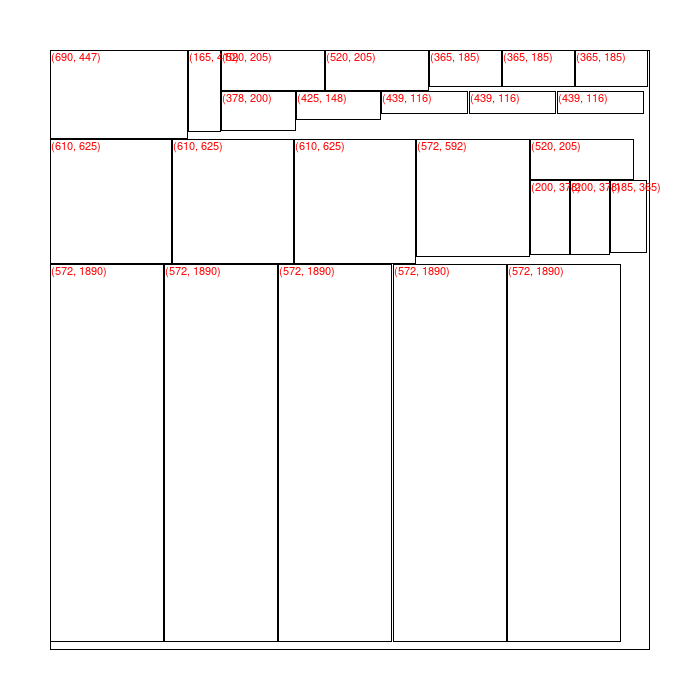
\includegraphics[width=1\linewidth]{results/cut13/2/cut}
  \label{fig:sub2}
\end{subfigure}
\caption{Instancia cut13.txt, Solução: 8296226, disperdício de 7.82\% de 3000x3000, {(296, 425): 1, (116, 439): 2, (425, 148): 2, (572, 1890): 5, (439, 116): 3, (970, 463): 1, (660, 490): 1, (1882, 549): 1, (205, 520): 1, (425, 296): 3}}
\label{fig:test}
\end{figure}


\begin{figure}
\centering
\begin{subfigure}{.5\textwidth}
  \centering
  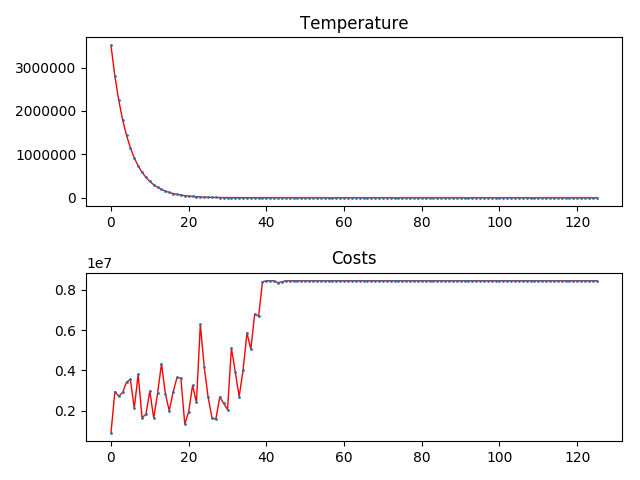
\includegraphics[width=1\linewidth]{results/cut14/2/plot}
  \label{fig:sub1}
\end{subfigure}%
\begin{subfigure}{.5\textwidth}
  \centering
  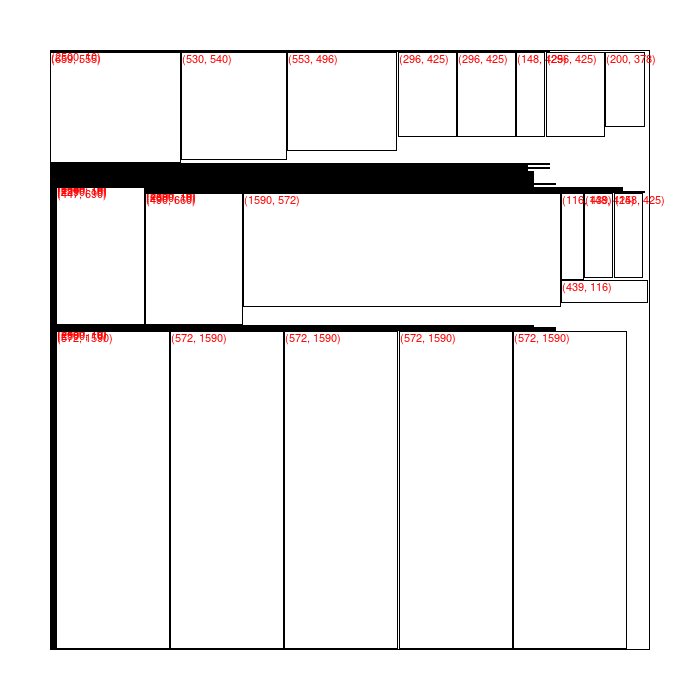
\includegraphics[width=1\linewidth]{results/cut14/2/cut}
  \label{fig:sub2}
\end{subfigure}
\caption{Instancia cut14.txt, Solução: 8443673, disperdício de 6.18\% de 3000x3000, {(555, 496): 1, (2500, 10): 1, (496, 555): 1, (10, 2390): 6, (447, 690): 1, (425, 148): 3, (660, 490): 1, (365, 185): 1, (949, 445): 1, (439, 116): 2, (378, 200): 1, (165, 410): 5, (530, 540): 3, (572, 1690): 5, (2390, 10): 6}}
\label{fig:test}
\end{figure}


\begin{figure}
\centering
\begin{subfigure}{.5\textwidth}
  \centering
  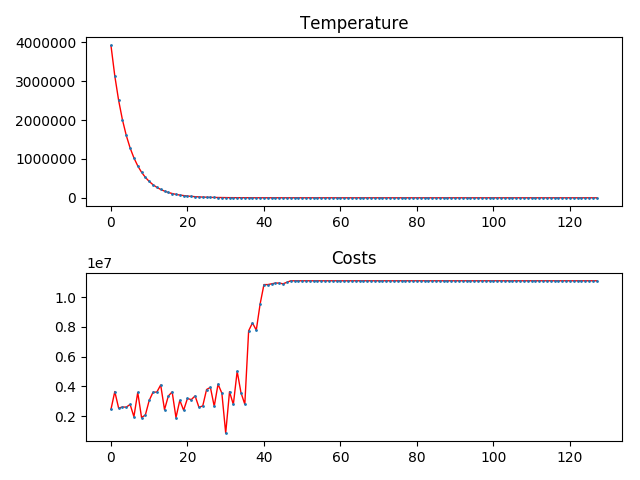
\includegraphics[width=1\linewidth]{results/cut17/2/plot}
  \label{fig:sub1}
\end{subfigure}%
\begin{subfigure}{.5\textwidth}
  \centering
  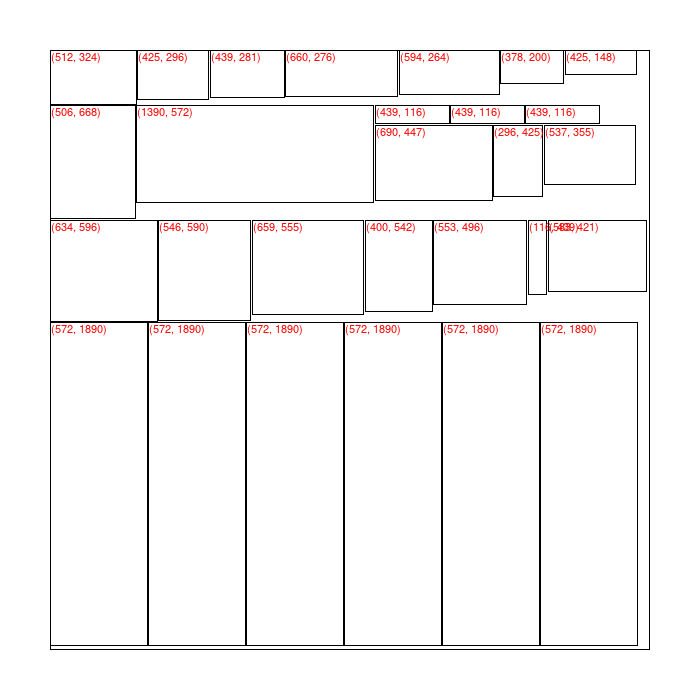
\includegraphics[width=1\linewidth]{results/cut17/2/cut}
  \label{fig:sub2}
\end{subfigure}
\caption{Instancia cut17.txt, Solução: 11142932, disperdício de 9.04\% de 3500x3500, {(405, 635): 1, (568, 625): 1, (400, 542): 1, (660, 276): 2, (483, 532): 1, (290, 605): 1, (278, 656): 1, (439, 116): 3, (410, 165): 1, (594, 264): 1, (116, 439): 1, (425, 148): 1, (290, 543): 1, (486, 320): 1, (1882, 549): 1, (352, 268): 1, (382, 323): 1, (549, 1882): 4, (327, 446): 1, (690, 447): 1, (572, 1690): 2, (599, 269): 1, (200, 378): 1}}
\label{fig:test}
\end{figure}


\begin{figure}
\centering
\begin{subfigure}{.5\textwidth}
  \centering
  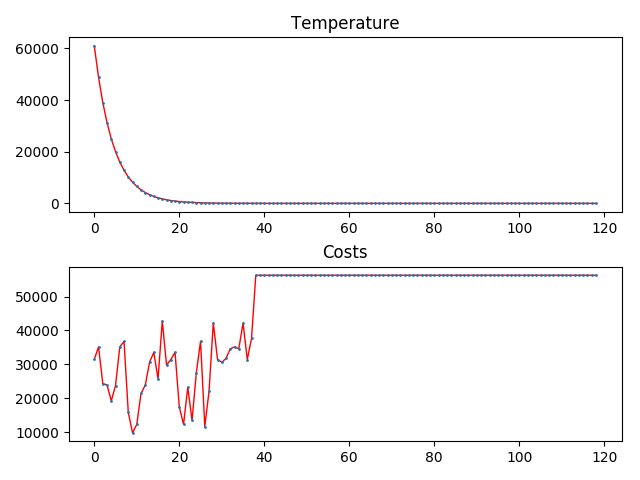
\includegraphics[width=1\linewidth]{results/cut1/1/plot}
  \label{fig:sub1}
\end{subfigure}%
\begin{subfigure}{.5\textwidth}
  \centering
  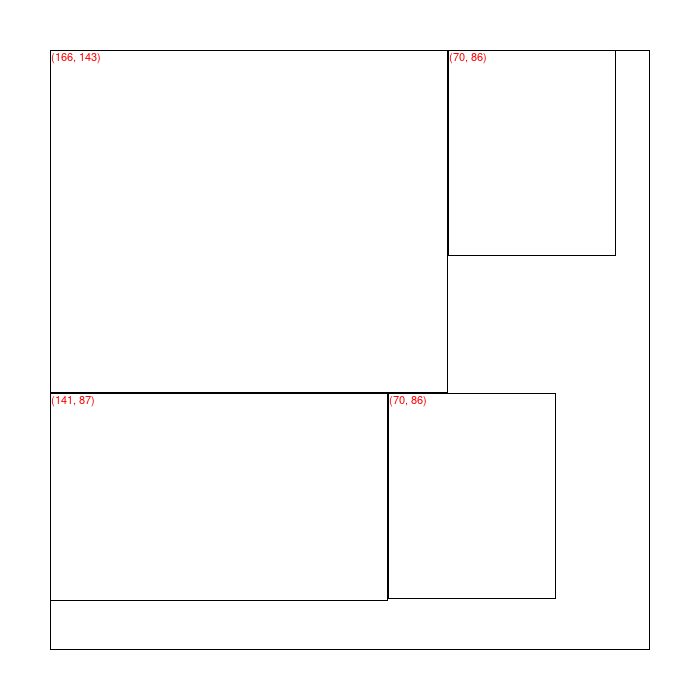
\includegraphics[width=1\linewidth]{results/cut1/1/cut}
  \label{fig:sub2}
\end{subfigure}
\caption{Instancia cut1.txt, Solução: 58136, disperdício de 6.98\% de 250x250, {(148, 66): 1, (83, 140): 1, (167, 184): 1}}
\label{fig:test}
\end{figure}


\begin{figure}
\centering
\begin{subfigure}{.5\textwidth}
  \centering
  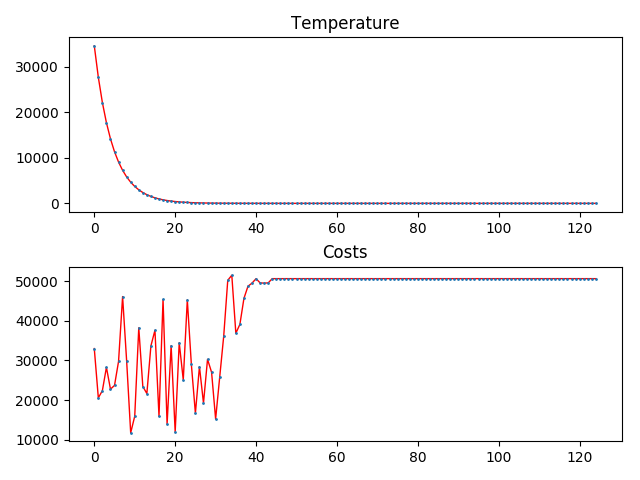
\includegraphics[width=1\linewidth]{results/cut2/2/plot}
  \label{fig:sub1}
\end{subfigure}%
\begin{subfigure}{.5\textwidth}
  \centering
  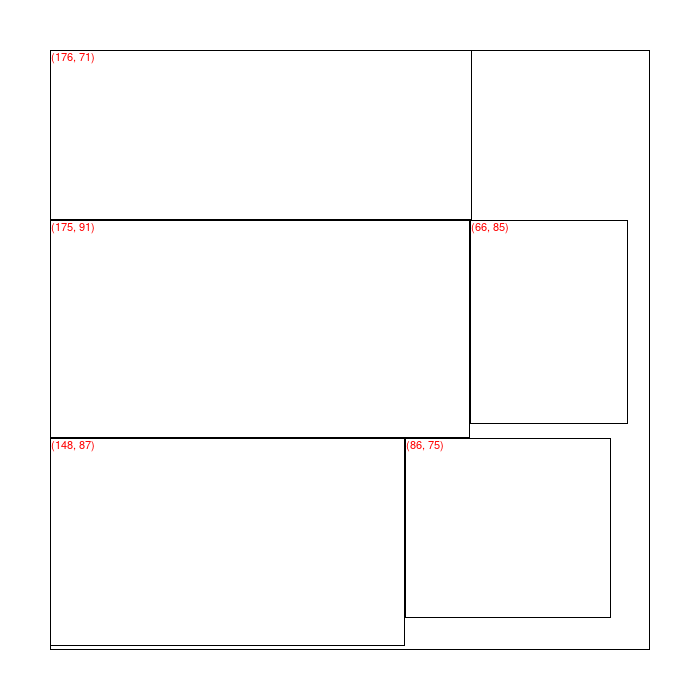
\includegraphics[width=1\linewidth]{results/cut2/2/cut}
  \label{fig:sub2}
\end{subfigure}
\caption{Instancia cut2.txt, Solução: 53357, disperdício de 14.63\% de 250x250, {(186, 135): 1, (168, 107): 1, (73, 103): 1}}
\label{fig:test}
\end{figure}


\begin{figure}
\centering
\begin{subfigure}{.5\textwidth}
  \centering
  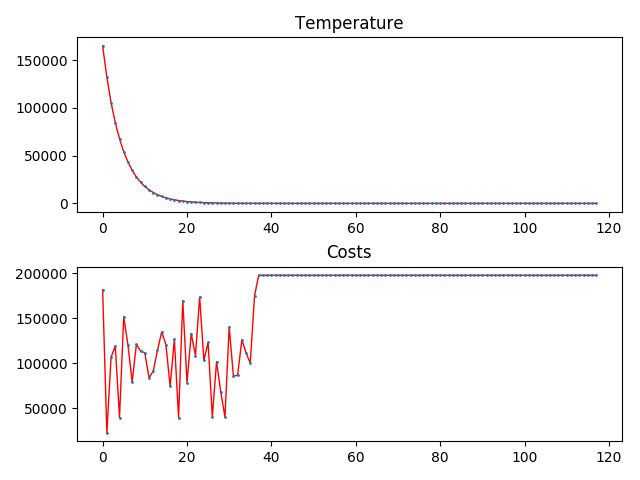
\includegraphics[width=1\linewidth]{results/cut5/2/plot}
  \label{fig:sub1}
\end{subfigure}%
\begin{subfigure}{.5\textwidth}
  \centering
  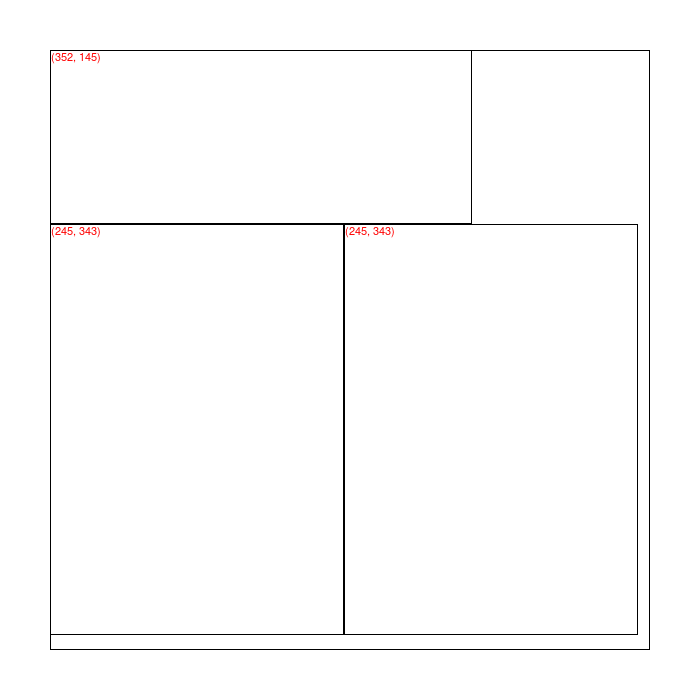
\includegraphics[width=1\linewidth]{results/cut5/2/cut}
  \label{fig:sub2}
\end{subfigure}
\caption{Instancia cut5.txt, Solução: 219110, disperdício de 12.36\% de 500x500, {(352, 145): 1, (145, 352): 1, (343, 245): 1}}
\label{fig:test}
\end{figure}


\begin{figure}
\centering
\begin{subfigure}{.5\textwidth}
  \centering
  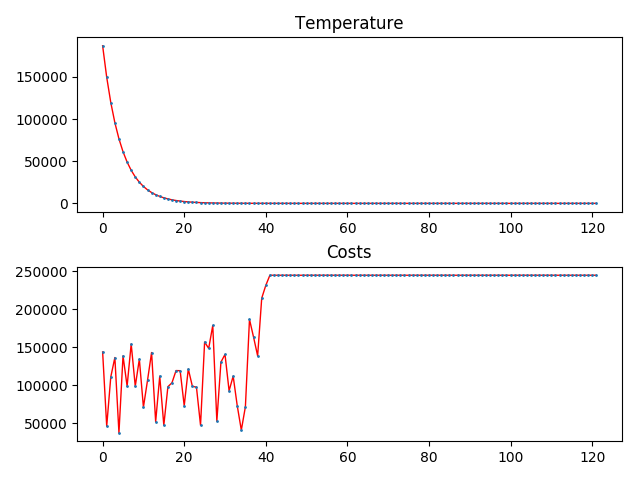
\includegraphics[width=1\linewidth]{results/cut7/1/plot}
  \label{fig:sub1}
\end{subfigure}%
\begin{subfigure}{.5\textwidth}
  \centering
  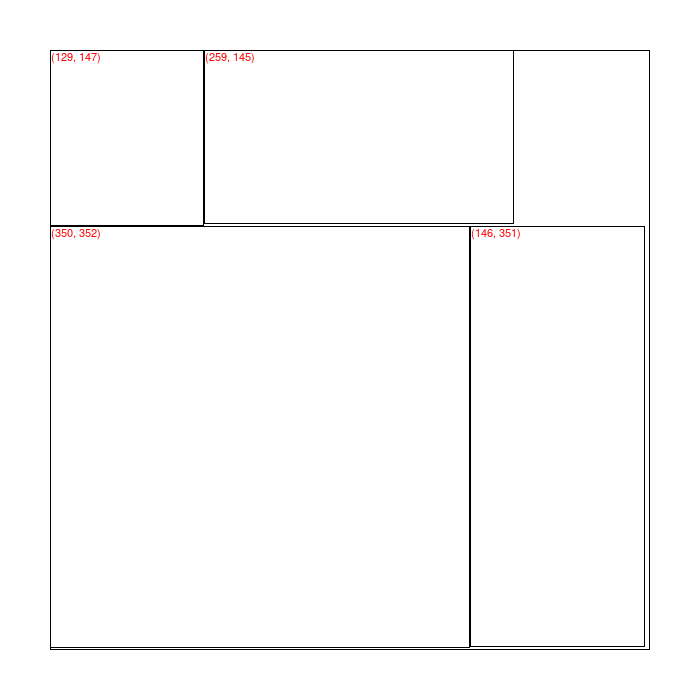
\includegraphics[width=1\linewidth]{results/cut7/1/cut}
  \label{fig:sub2}
\end{subfigure}
\caption{Instancia cut7.txt, Solução: 244655, disperdício de 2.14\% de 500x500, {(348, 322): 1, (145, 259): 1, (129, 147): 1, (369, 171): 1}}
\label{fig:test}
\end{figure}


\begin{figure}
\centering
\begin{subfigure}{.5\textwidth}
  \centering
  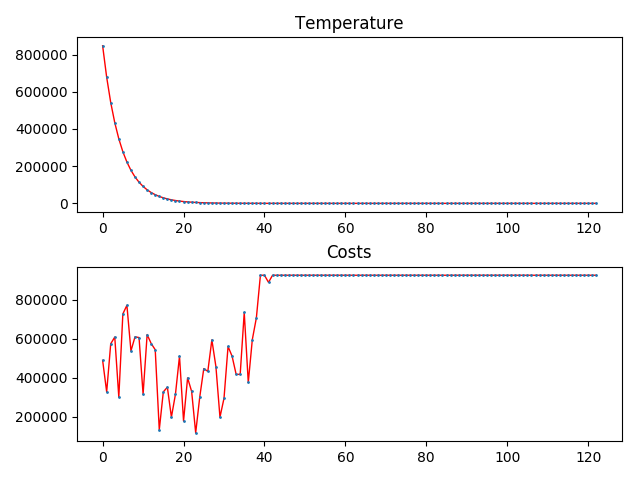
\includegraphics[width=1\linewidth]{results/cut9/3/plot}
  \label{fig:sub1}
\end{subfigure}%
\begin{subfigure}{.5\textwidth}
  \centering
  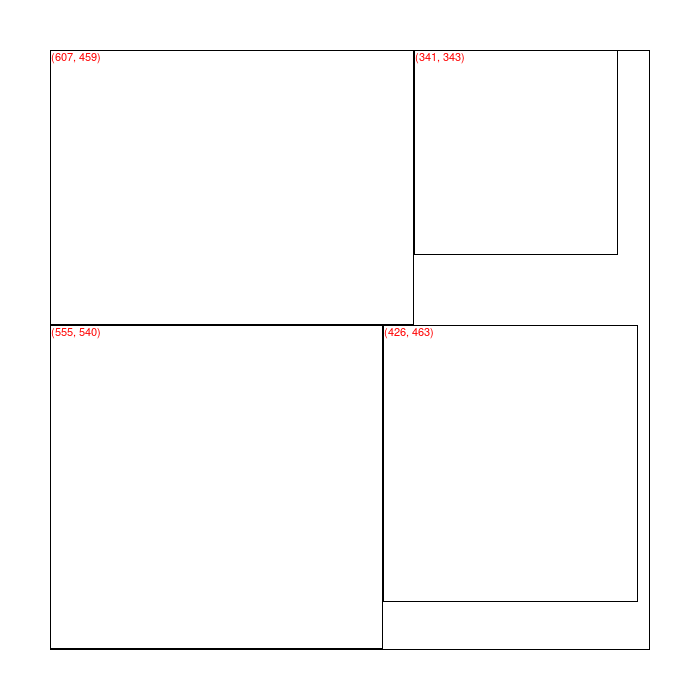
\includegraphics[width=1\linewidth]{results/cut9/3/cut}
  \label{fig:sub2}
\end{subfigure}
\caption{Instancia cut9.txt, Solução: 953628, disperdício de 4.64\% de 1000x1000, {(498, 325): 2, (468, 673): 2}}
\label{fig:test}
\end{figure}


\begin{figure}
\centering
\begin{subfigure}{.5\textwidth}
  \centering
  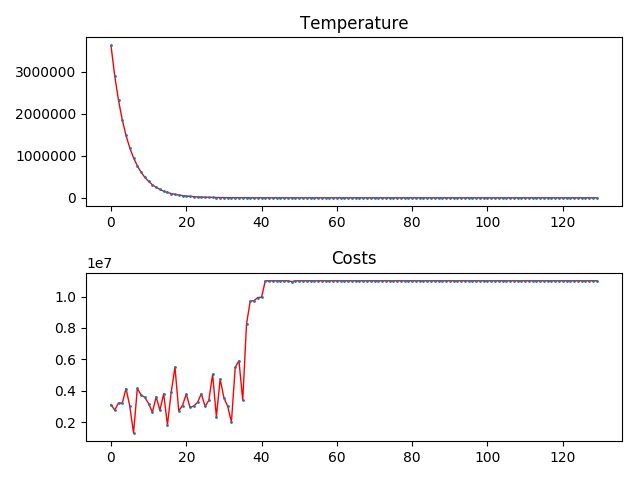
\includegraphics[width=1\linewidth]{results/livre/2/plot}
  \label{fig:sub1}
\end{subfigure}%
\begin{subfigure}{.5\textwidth}
  \centering
  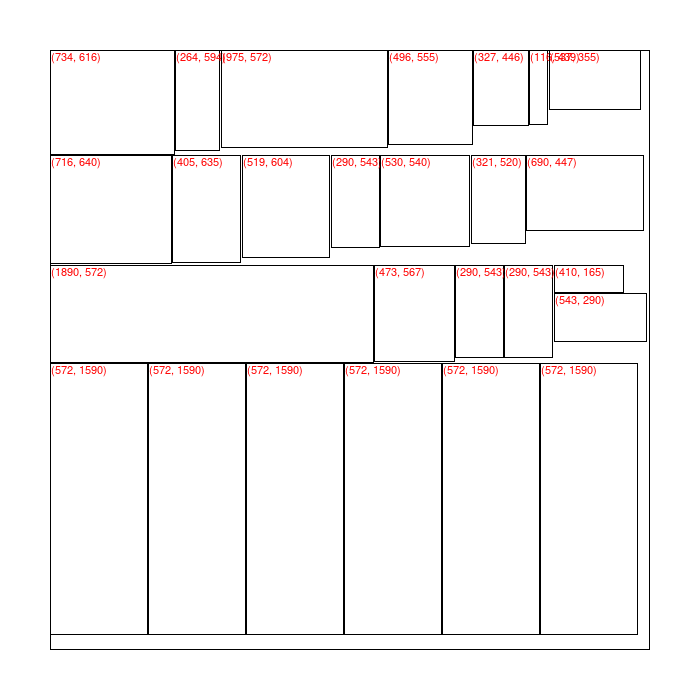
\includegraphics[width=1\linewidth]{results/livre/2/cut}
  \label{fig:sub2}
\end{subfigure}
\caption{Instancia livre.txt, Solução: 11002738, disperdício de 10.18\% de 3500x3500, {(555, 496): 1, (528, 459): 1, (696, 497): 1, (421, 583): 2, (526, 273): 1, (572, 1590): 6, (378, 200): 1, (410, 165): 1, (606, 479): 1, (530, 540): 1, (479, 606): 2, (352, 268): 1, (365, 185): 1, (678, 414): 1, (512, 324): 1, (519, 604): 1, (414, 678): 1, (426, 579): 1, (665, 572): 2, (339, 405): 1}}
\label{fig:test}
\end{figure}

